\begin{figure}
  \setlength{\unitlength}{\textwidth}

        \begin{picture}(1,0.4)(0,0.4)

      \put(0.1,0.45){\includegraphics[width=0.75\unitlength]{../FnP/gnuplot/spec_pow.eps}}
      
%       \put(0.07,0.95){$\displaystyle\frac{V}{D}$}
%       \put(0.07,1.3){$\displaystyle\frac{A}{D}$}
       \put(0.045,0.455){\rotatebox{90}{Relative power of shedding }}
%       \put(0.5,0.4){$\massdamp$}
       \put(0.46,0.4){$\massstiff$}
    \end{picture}

  % \caption{Comparison of maximum power between QSS and DNS data obtained using 3 point local quadratic curve fitting.The error was obtained using Eq:\ref{eqn:error_calculation}}
    \caption{The relative power of the vortex shedding as a fucntion of \massstiff. The relative power of the vortex shedding decreases as \massstiff \ increases. The dash curve (\protect\dashedrule) follows the power low fit of the percentage error which is $f(x)=0.977x^{-0.52} $ equation.}
    \label{fig:spec_pow}
\end{figure}

 %vspace{10cm}
